\section{Evaluation}
\label{sec:evaluation}

\vv{estes testes incluem o tempo de parsing? nao deveriam. deveriam só
  contar o tempo da chamada à funcao bisimilar/equivalent.}

% In this section, we analyze the performance of our algorithm
% to check the equivalence of context-free session types. 
% To do so, 
We implemented the algorithm
% we have presented thus far (sketched in
% Listings~\ref{lst:toGrammar}, \ref{lst:prune}, \ref{lst:algorithm})
in Haskell and used the Glasgow Haskell Compiler, GHC version 8.6.3,
from which we have obtained the running times we present in this
section.  Evaluation was conducted on a Mac mini equipped with a 3.6
GHz Intel Core i3, 8 GB of memory, and running MacOS 10.14.3.
%
Armed with the results in section~\ref{sec:algorithm}, we decided to
benchmark the algorithm on a test suite of carefully crafted pair of
types. During this process we came across a pair of types,
\begin{equation}
\label{ex:chaotic}
\begin{aligned}
  S &\triangleq \mu x . \&\{ \mathsf{Add}\colon x;x; !\,\intk,
  \mathsf{Const}\colon ?\,\intk;!\intk,
  \mathsf{Mult}\colon x;x;!\,\intk\}
  \\
  T &\triangleq \mu x . \&\{ \mathsf{Add}\colon x;x,
  \mathsf{Const}\colon ?\,\intk,
  \mathsf{Mult}\colon x;x\}; !\,\intk
\end{aligned}
\end{equation}
%
on which function \lstinline|bisimilar| took 4379.98 seconds (that is
one hour and forty minutes) to terminate. This is certainly not a
reasonable running time for an algorithm to be included in a
compiler. Hence, we looked into ways to improve the running
times. Among the different optimisations that we tried, two stand
out:
\begin{enumerate}
\item Iterate the simplification stage until a fixed point is reached;
\item Use a double-ended queue where promising children is prepended
  rather than appended.
\end{enumerate}

If, on the one hand, we believed that the computation of the expansion
tree could be speeded up by extending the simplification phase, on the
other hand we suspected that a double-ended queue would allow
prioritizing nodes with potential to reach an empty node faster.  The
latter is obtained by prepending nodes that are already empty or,
either, whose pairs $(\vec X, \vec Y)$ are such that $|\vec X|\leq 1$
and $|\vec Y| \leq 1$.  For the former, we need to check that a fixed
point exists and, hence, for a given node $N$, we are able to compute
the \emph{simplest} children nodes derived from $N$ using the
simplification rules.


We have tested the several combination of the previous proposals
in our algorithm on a batch of 138 tests. The results are presented 
in Figure~\ref{fig:results}.

\begin{figure}[h]
	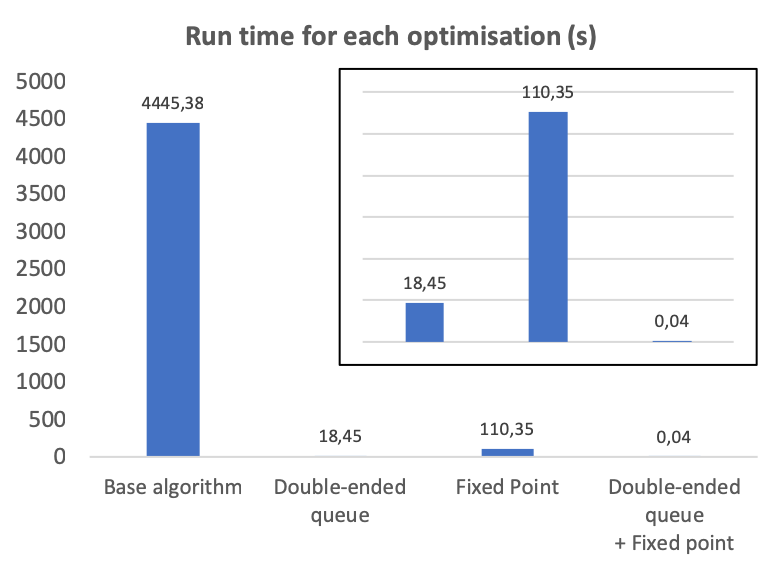
\includegraphics[height=4.8cm]{img/run_time}	\qquad 
	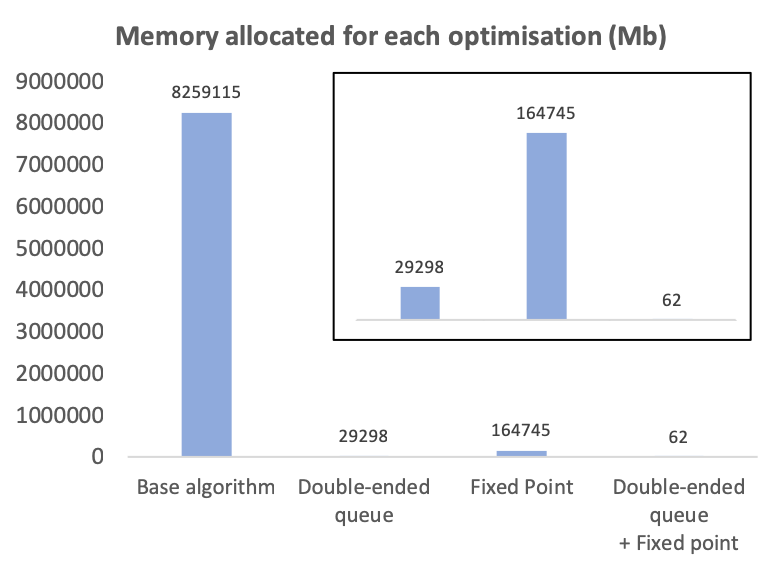
\includegraphics[height=4.8cm]{img/memory_alloc}	
	\caption{Test results: running times (on the left) and
	memory allocated (on the right) checking the equivalence 
	of context-free session types in 138 tests.}
	\label{fig:results}
\end{figure}

The running times and memory allocated are presented in
Figure~\ref{fig:results}, exhibit an improvement on more than
12,000,000\%. The running time of example in~\eqref{ex:chaotic} was
brought down to 0.01 seconds \vv{talvez seja ainda menos. as
  centesimas parecem ser a resolucao maxima do haskell; que tal correr
  o mesmo teste 100 vezes e dividir por 100?} For this reasons, our
proposal for an algorithm to check the equivalence of context-free
session types stands on adapting the simplification stage to enable
double-ended enqueueing and the computation of a fixed point at the
simplification phase Listing~\ref{lst:enhanced} presents an enhanced
version of the simplification stage coping the new proposals.



%%% Local Variables:
%%% mode: latex
%%% TeX-master: "main"
%%% End:
